\documentclass{beamer}
\usepackage{tikz}
\usepackage{hyperref}
 
\title{\href{https://hexdocs.pm/phoenix/Phoenix.html}{Phoenix Framework}}
\author{\href{https://github.com/WannesFransen1994}{Wannes Fransen} \& \href{https://github.com/TomEversdijk}{Tom Eversdijk}}
\institute{\href{https://www.ucll.be}{UC Leuven}}
 \date{2021}
 

\begin{document}

\frame{\titlepage}


\section{The Phoenix framework}

\frame{\tableofcontents[currentsection]}

\begin{frame}
    \frametitle{Why a framework?}
    \begin{itemize}
        \item Avoid writing the same code over and over again
        \item Higher interopability between your code \& boilerplate code
        \item Abstractions to e.g. sessions, security, databases, etc...
        \item Other developers can focus on the important bits
    \end{itemize}
\end{frame}

\begin{frame}
    \frametitle{What is Phoenix?}
    \begin{itemize}
        \item Web development framework written in Elixir
        \item Inspired by concepts of Ruby on Rails
        \item Server Side MVC framework
        \item High performance \& made for realtime features
        \item Great language/framework for long connections
    \end{itemize}
\end{frame}
\section{Phoenix internals}

\frame{\tableofcontents[currentsection]}

\begin{frame}
    \frametitle{Phoenix layers}
    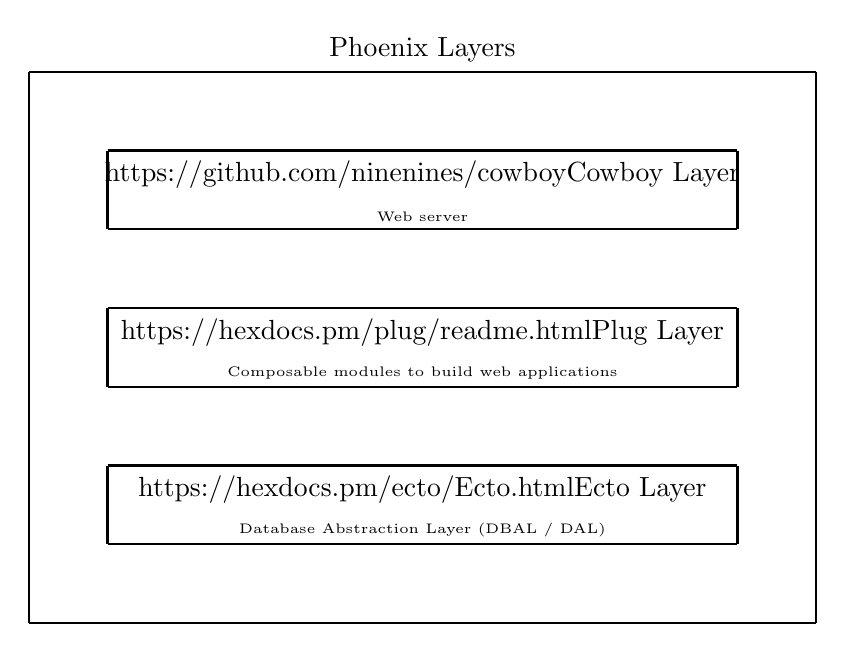
\begin{tikzpicture}
        % TODO: refactor https://www.overleaf.com/learn/latex/LaTeX_Graphics_using_TikZ:_A_Tutorial_for_Beginners_(Part_1)%E2%80%94Basic_Drawing
        % ############### OUTER BOX START ##################
        % Upper horizontal line with phoenix text
        \draw[thick] (0,2) -- node[above] {Phoenix Layers} (10,2);
        % Lower horizontal line
        \draw[thick] (0,-5) -- (10,-5);

        % Left vertical line
        \draw[thick] (0,2) -- (0,-5);
        % Right vertical line
        \draw[thick] (10,2) -- (10,-5);

        % ############### OUTER BOX END ####################

        % ############### LAYER COWBOY START ###############
        % Upper horizontal line with cowboy layer
        \draw[thick] (1,1) -- node[below] {\href{https://github.com/ninenines/cowboy}{Cowboy Layer}} (9,1);
        % Lower horizontal line
        \tiny
        \draw[thick] (1,0) -- node[above] {Web server} (9,0);
        \normalsize
        % Left vertical line
        \draw[thick] (1,1) -- (1,0);
        % Right vertical line
        \draw[thick] (9,1) -- (9,0);
        % ############### LAYER COWBOY END #################

        % ############### LAYER PLUG START #################
        % Upper horizontal line with plug layer
        \draw[thick] (1,-1) -- node[below] {\href{https://hexdocs.pm/plug/readme.html}{Plug Layer}} (9,-1);
        % Lower horizontal line
        \tiny
        \draw[thick] (1,-2) -- node[above] {Composable modules to build web applications} (9,-2);
        \normalsize
        % Left vertical line
        \draw[thick] (1,-1) -- (1,-2);
        % Right vertical line
        \draw[thick] (9,-1) -- (9,-2);
        % ############### LAYER PLUG END ###################

        % ############### LAYER ECTO START #################
        % Upper horizontal line with Ecto layer
        \draw[thick] (1,-3) -- node[below] {\href{https://hexdocs.pm/ecto/Ecto.html}{Ecto Layer}} (9,-3);
        % Lower horizontal line
        \tiny
        \draw[thick] (1,-4) -- node[above] {Database Abstraction Layer (DBAL / DAL)} (9,-4);
        \normalsize
        % Left vertical line
        \draw[thick] (1,-3) -- (1,-4);
        % Right vertical line
        \draw[thick] (9,-3) -- (9,-4);
        % ############### LAYER ECTO END ###################
    \end{tikzpicture}
\end{frame}


\begin{frame}
    \frametitle{\href{https://hexdocs.pm/phoenix/request_lifecycle.html}{Request lifecycle}}
    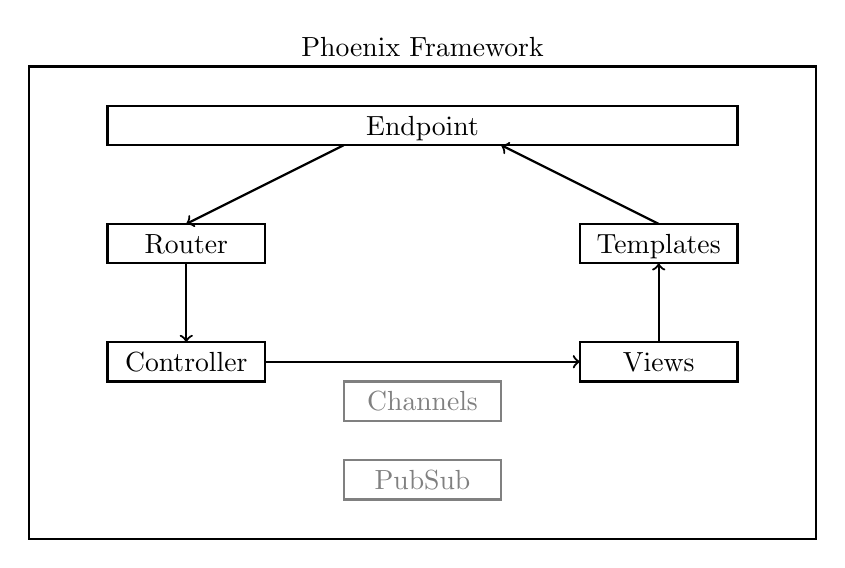
\begin{tikzpicture}

        \draw[thick] (0,2) -- node[above] {Phoenix Framework}
        (10,2) -- (10,-4) -- (0,-4) -- cycle;

        \draw[thick] (1,1.5) -- node[below] {Endpoint}
        (9,1.5) -- (9,1) -- (1,1) -- cycle;

        \draw[thick] (1,0) -- node[below] {Router}
        (3,0) -- (3,-0.5) -- (1,-0.5) -- cycle;

        \draw[thick] (1,-1.5) -- node[below] {Controller}
        (3,-1.5) -- (3,-2) -- (1,-2) -- cycle;

        \draw[thick] (7,-1.5) -- node[below] {Views}
        (9,-1.5) -- (9,-2) -- (7,-2) -- cycle;

        \draw[thick] (7,-0) -- node[below] {Templates}
        (9,-0) -- (9,-0.5) -- (7,-0.5) -- cycle;

        \draw[thick, gray] (4,-2) -- node[below] {Channels}
        (6,-2) -- (6,-2.5) -- (4,-2.5) -- cycle;

        \draw[thick, gray] (4,-3) -- node[below] {PubSub}
        (6,-3) -- (6,-3.5) -- (4,-3.5) -- cycle;

        % #######################################

        \draw[->, thick] (4,1) -- (2,0);
        \draw[->, thick] (2,-0.5) -- (2,-1.5);
        \draw[->, thick] (3,-1.75) -- (7,-1.75);
        \draw[->, thick] (8,-1.5) -- (8,-0.5);
        \draw[->, thick] (8,0) -- (6,1);

    \end{tikzpicture}
\end{frame}

\begin{frame}
    \frametitle{Websocket communication (soft-realtime)}
    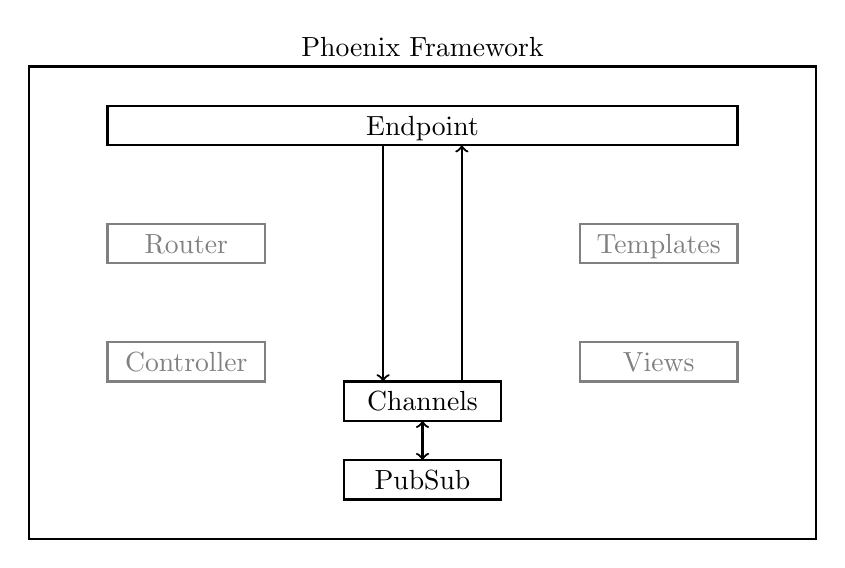
\begin{tikzpicture}

        \draw[thick] (0,2) -- node[above] {Phoenix Framework}
        (10,2) -- (10,-4) -- (0,-4) -- cycle;

        \draw[thick] (1,1.5) -- node[below] {Endpoint}
        (9,1.5) -- (9,1) -- (1,1) -- cycle;

        \draw[thick, gray] (1,0) -- node[below] {Router}
        (3,0) -- (3,-0.5) -- (1,-0.5) -- cycle;

        \draw[thick, gray] (1,-1.5) -- node[below] {Controller}
        (3,-1.5) -- (3,-2) -- (1,-2) -- cycle;

        \draw[thick, gray] (7,-1.5) -- node[below] {Views}
        (9,-1.5) -- (9,-2) -- (7,-2) -- cycle;

        \draw[thick, gray] (7,-0) -- node[below] {Templates}
        (9,-0) -- (9,-0.5) -- (7,-0.5) -- cycle;

        \draw[thick] (4,-2) -- node[below] {Channels}
        (6,-2) -- (6,-2.5) -- (4,-2.5) -- cycle;

        \draw[thick] (4,-3) -- node[below] {PubSub}
        (6,-3) -- (6,-3.5) -- (4,-3.5) -- cycle;

        % #######################################

        \draw[->, thick] (4.5,1) -- (4.5,-2);
        \draw[->, thick] (5.5,-2) -- (5.5,1);

        \draw[->, thick] (5,-2.5) -- (5,-3);
        \draw[->, thick] (5,-3) -- (5,-2.5);

    \end{tikzpicture}
\end{frame}

\begin{frame}
    \frametitle{Libraries explanation 1/3}
    \structure{Endpoint}
    \begin{itemize}
        \item start and end of the request lifecycle
        \item all aspects of requests up until the router takes over
        \item core set of plugs to apply to all requests
    \end{itemize}

    \vfill

    \structure{Router}
    \begin{itemize}
        \item parses and dispatches requests to the correct controller/action
        \item helpers to generate route paths or urls to resources
        \item pipelines - applies groups of plugs to a set of routes
    \end{itemize}

    \vfill

    \structure{Controller}
    \begin{itemize}
        \item provide functions, called actions, to handle requests
        \item action: prepare data and pass it into views
        \item action: invoke rendering via views 
        \item action: perform redirects 
    \end{itemize}
\end{frame}

\begin{frame}
    \frametitle{Libraries explanation 2/3}
    \structure{Views - presentation layer}
    \begin{itemize}
        \item render templates
        \item define template helper functions to decorate data
    \end{itemize}

    \vfill

    \structure{Templates}
    \begin{itemize}
        \item files containing the contents that will be served in a response
        \item basic response structure, allow dynamic data to be inserted
        \item precompiled and fast
    \end{itemize}
\end{frame}

\begin{frame}
    \frametitle{Libraries explanation 3/3}

    \structure{Channels}
    \begin{itemize}
        \item manage sockets for easy realtime communication
        \item analogous to controllers, but allow bi-directional communication with persistent connections
    \end{itemize}

    \vfill

    \structure{PubSub}
    \begin{itemize}
        \item underlies the channel layer and allows clients to subscribe to topics
    \end{itemize}
\end{frame}
\section{Mix}

\frame{\tableofcontents[currentsection]}

\begin{frame}
    \frametitle{What is mix?}   
    \begin{itemize}
        \item Build tool
        \item Create your application 
        \item compile / test your code
        \item Dependency management
        \item Custom commands
        \item Configuration management
        \item ...
    \end{itemize}
\end{frame}

\begin{frame}
    \frametitle{Sample usage}   
    \begin{itemize}
        \item mix new sample\_application (- - sup)
        \item mix phx.new application\_name (- - no-html, - - database)
        \vfill        
        \item mix run
        \item mix test
        \item mix compile
        \item mix deps.get
        \item mix deps.compile
    \end{itemize}
\end{frame}
\section{Project structure}

\frame{\tableofcontents[currentsection]}

\begin{frame}
    \frametitle{Basic mix project structure}   
    \structure{Umbrella projects} \\
    Instead of building a single large monolith, you can structure your code with multiple isolated contexts.
    \begin{itemize}
        \item poor man’s microservices solution
        \item compiled and run under the same BEAM instance
        \item Dependencies between applications must be explicitly defined
        \item Degree of separation, not fully decoupled!
    \end{itemize}
    \vfill
    \small
    Different configurations in each application for the same dependency or use different dependency versions, then it is likely your codebase has grown beyond what umbrellas can provide.
\end{frame}

\begin{frame}[fragile]
    \frametitle{Sample generated project - umbrella structure}   
    mix phx.new demo --umbrella --database mysql
    \vfill
    \begin{verbatim}
    hello_umbrella
    |-- _build
    |-- apps
    |   |-- hello               => domain application
    |   |   |-- ...
    |   |-- hello_web           => web application
    |   |   |-- ...
    |-- config                  => shared config
    |-- deps
    \end{verbatim} 
\end{frame}

\begin{frame}[fragile]
    \frametitle{Sample generated project - domain structure}
    \begin{verbatim}
    hello
    |-- lib
    |   |-- hello
    |   |   |-- foo_context     => context folder
    |   |   |   |-- foo.ex      => foo-related modules
    |   |   |-- foo_context.ex  => context module
    |   |   |-- application.ex  => starts app processes
    |   |   |-- repo.ex         => module for db operations
    |   |   |-- ...
    |   |-- hello.ex            => app interface
    |-- priv
    |   |-- repo
    |   |   |-- migrations
    |   |   |-- seeds.ex        => default data in your db
    |   |   |-- ...
    |-- test
    |   |-- ...
\end{verbatim} 
\end{frame}

\begin{frame}[fragile]
    \frametitle{Sample generated project - web structure}

    \begin{verbatim}
    hello_web
    |-- controllers
    |   |-- foo_controller.ex
    |   |-- bar_controller.ex
    |-- templates
    |   |-- foo
    |   |   |-- index.html.eex
    |   |   |-- ...
    |   |-- bar
    |   |   |-- index.html.eex
    |   |   |-- ...
    |-- views
    |   |-- foo_view.ex
    |   |-- bar_view.ex
    \end{verbatim} 

\end{frame}

\begin{frame}
    \frametitle{General guidelines}

    \begin{itemize}
        \item No domain code in controller
        \item No direct usage of Repo in your web project
        \item Controllers will use Contexts to communicate with your domain
    \end{itemize}

\end{frame}
\section{Getting started with routing}

\frame{\tableofcontents[currentsection]}

\begin{frame}
    \frametitle{\href{https://devhints.io/phoenix-routing}{Routing}}

    \begin{itemize}
        \item Match HTTP requests to controller actions
        \item \href{https://hexdocs.pm/phoenix/routing.html\#nested-resources}{Nested resources} - create nested requests automatically
        \item \href{https://hexdocs.pm/phoenix/routing.html\#scoped-routes}{Scoped routes} - group routes under a common path prefix and scoped set of plugs
        \item \href{https://hexdocs.pm/phoenix/routing.html\#path-helpers}{Path helpers} - ensure our controllers, views and templates are linking to pages our router can actually handle sure
    \end{itemize}
\end{frame}


\section{Getting started with Ecto}

\frame{\tableofcontents[currentsection]}

\begin{frame}
    \frametitle{Ecto - the concepts}

    \begin{itemize}
        \item Repo module - Via the repository, we can create, update, destroy and query existing entries.
        \item Schemas - used  to map data sources to Elixir structs.
        \item Changesets - way to filter and cast external parameters, as well to validate changes before applying them
        \item Query - queries written in Elixir syntax with specific DSL. Queries are by default secure, avoiding common problems. These can be created composable / piece by piece
    \end{itemize}
\end{frame}

\begin{frame}
    \frametitle{Ecto SQL - not the same thing!}

    \begin{itemize}
        \item This provides functionality for working with SQL databases in Ecto
        \item Migrations are an example of this
    \end{itemize}
\end{frame}

\begin{frame}[fragile]
    \frametitle{There's already a great guide for this}

    \begin{itemize}
        \item Database is up to you (MySQL might be the easiest)
        \item Feel free to use generators such as:
        \begin{verbatim}
mix phx.gen.schema User users \ 
name:string email:string \
bio:string number_of_pets:integer
        \end{verbatim}
    \end{itemize}

    \vfill

    \href{https://hexdocs.pm/phoenix/ecto.html\#content}{[LINK]}
\end{frame}
\section{Exercises}

\frame{\tableofcontents[currentsection]}

\begin{frame}
    \frametitle{Exercises}
    \begin{itemize}
        \item \href{https://hexdocs.pm/phoenix/installation.html\#node-js}{Install NodeJS}
        \item Task 1: Make a new (static) page
        \item Task 2: Make a new page with a random number on item 
        \item Task 3: Implement CRUD for a single entity \footnotemark[1]
        \item Task 4: Link 2 entities \footnotemark[1]
    \end{itemize}

    \href{https://elixirforum.com/t/visual-studio-code-html-eex-support/12712/5}{Tip: treat .eex files as html}
    \footnotetext[1]{Seen next lesson} 

\end{frame}

\section{Links}

\frame{\tableofcontents[currentsection]}

\begin{frame}
    \frametitle{Links}
    \begin{itemize}
        \item \href{https://hexdocs.pm/phoenix/Phoenix.html}{Phoenix Framework}
        \item \href{https://hexdocs.pm/phoenix/request_lifecycle.html}{Request lifecycle}
        \item \href{https://devhints.io/phoenix-routing}{Routing}
        \begin{itemize}
            \item \href{https://hexdocs.pm/phoenix/routing.html\#nested-resources}{Nested resources}
            \item \href{https://hexdocs.pm/phoenix/routing.html\#scoped-routes}{Scoped routes}
            \item \href{https://hexdocs.pm/phoenix/routing.html\#path-helpers}{Path helpers}
        \end{itemize}
        \item \href{https://hexdocs.pm/phoenix/ecto.html}{Ecto}
        \begin{itemize}
            \item \href{https://hexdocs.pm/phoenix/ecto.html\#repo-configuration}{Repo configuration}
            \item \href{https://hexdocs.pm/phoenix/ecto.html\#the-schema}{Schemas}
            \item \href{https://hexdocs.pm/phoenix/ecto.html\#changesets-and-validations}{Changesets and validations} 
        \end{itemize}
    \end{itemize}
\end{frame}




\end{document}

